\documentclass[12pt, letterpaper, a4paper]{article}
\usepackage{graphicx}
\usepackage{textcomp}
\usepackage[hungarian]{babel}
\usepackage[T1]{fontenc}
\usepackage[utf8]{inputenc}
\usepackage{caption}
\usepackage{subcaption}
\usepackage{csquotes}
\graphicspath{{./images/}}
\usepackage[
    style=ieee,
  ]{biblatex}
\addbibresource{soc.bib}

\usepackage{listings}
\usepackage[svgnames]{xcolor}
\usepackage{tikz}
\usetikzlibrary{shapes.geometric, arrows}

\definecolor{dkgreen}{rgb}{0,0.6,0}
\definecolor{gray}{rgb}{0.5,0.5,0.5}
\definecolor{mauve}{rgb}{0.58,0,0.82}

\lstset{frame=tb,
  language=Bash,
  aboveskip=3mm,
  belowskip=3mm,
  showstringspaces=false,
  columns=flexible,
  basicstyle={\small\ttfamily},
  numbers=none,
  numberstyle=\tiny\color{gray},
  keywordstyle=\color{blue},
  commentstyle=\color{dkgreen},
  stringstyle=\color{mauve},
  breaklines=true,
  breakatwhitespace=true,
  tabsize=2
}

\tikzstyle{startstop} = [rectangle, rounded corners, minimum width=3cm, minimum height=1cm,text centered, draw=black, fill=red!30]
\tikzstyle{arrow} = [thick,->,>=stealth]


\title{\textcolor{RoyalBlue}{\textbf{Heterogén SoC rendszerek házi feladat}}}
\author{\textcolor{RoyalBlue}{Batcher Odd-Even-Merge algoritumus skalár megvalósítás} \\ \\ Nyiri Levente}
\date{2025 Október}
\begin{document}
\selectlanguage{hungarian}
\maketitle

\newpage

\section{Algoritmus}

Batcher Odd-Even-Merge algoritmusa úgy műdödik, hogy elfelezzük a listánkat, külön-külön rendezzük a feleket, majd a páros és páratlan indexű elemeket is összehasonlítjuk. Ezután már csak egyszer kell a szomszédos elemeket összehasonlítani és a számhalmunk rendezve van.

Ez egy rekurzív algoritmus. Két részből áll: egy olyan algoritmus ami a két rendezett felet kialakítja (sort), és egy olyan ami ezeket a rendezett feleket felhasználva rendez tovább (merge).

\subsection{sort}

A tömbünk hosszát elosztjuk 2-vel, \( m = \frac{lenght}{2} \), majd ezt átadva hosszként újra meghívjuk a függvényt. Ismét meghívjuk afüggvényt, ezúttal a kezdeti pontot \(m\)-el eltolva. Végül meghívjuk a merge függvényt, ami abban az esetben ha csak két elemet adunk át, akkor összehasonlítja és szükség esetén megcseréli őket. Hosszabb lista esetén ő is rekurzívan működik, először meghívja önmagát 0-ás indextől kezdve, majd ismét, 1-es indextől. A következő lépése, hogy összehasonlítsa az átadott lista páratlan indexű elemeit.
%TODO: ezt átírni kevésbé katyvaszosra

A működést legjobban rekurzív algoritmusoknál szerintem call stack-el lehet szemléltetni, ez látható a \ref{fig:call-stack}.-ik ábrán.


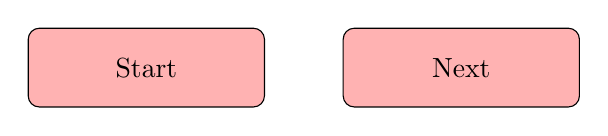
\begin{tikzpicture}[node distance=2cm]
  \node (start) [startstop] {Start};

  \node (next) [startstop, right of=start, xshift=2cm] {Next};
\end{tikzpicture}


\end{document}
